\documentclass[12pt,a4paper]{article}
\usepackage[utf8]{vietnam}
\usepackage{amsmath,amssymb}
\usepackage{tabularx}
\usepackage{tikz}
\usepackage{xcolor}
\usepackage[top=0.6cm, bottom=0.6cm, left=0.6cm, right=0.6cm]{geometry}
\usepackage[dethi]{ex_test}

\SAOPTN{widthSA=2.8,heightSA=0.62}
\setlength{\parskip}{0pt}

% Dong ke cham mo chuan viet tay
\newcommand{\dongke}[1]{%
  \begingroup%
  \setlength{\parskip}{0pt}%
  \baselineskip=18.5pt%
  \vspace{1.0mm}%
  \foreach \i in {1,...,#1}{%
    \noindent{\color{gray!60}\dotfill}\par%
  }%
  \vspace{0.6mm}%
  \endgroup%
}

% Khu vuc bai lam chia 2 cot co vach ngan mo o giua
\newcommand{\dongkeHaiCot}[1]{%
  \par\vspace{0.5mm}%
  \noindent%
  \begin{minipage}[t]{0.485\linewidth}%
    \dongke{#1}%
  \end{minipage}%
  \hfill%
  {\color{gray!60}\vrule}%
  \hfill%
  \begin{minipage}[t]{0.485\linewidth}%
    \dongke{#1}%
  \end{minipage}%
}

% Dinh nghia o bai tap tu luan trong bang
\newcommand{\oBaiTap}[3][5]{%
  \vspace{1.0mm}%
  \noindent\textbf{#2} #3\par%
  \dongke{#1}%
}

\begin{document}
\pagestyle{empty}
% =============================================================================
% ========================= TOAN 8 TUAN 11 BUOI 01 - MA DE 101 =================
% ========================= TRANG 1/2 ==========================================
% =============================================================================
\noindent
\begin{tabularx}{\linewidth}{|X|c|}
\hline
\textbf{PHIẾU KIỂM TRA ĐỊNH KỲ TOÁN 8 - TUẦN 11 - BUỔI 01} & \textbf{Mã đề: 101 - Trang 1/2} \\
\hline
\end{tabularx}

\vspace{1.0mm}

\noindent
\begin{tabularx}{\linewidth}{|p{3.2cm}|X|}
\hline
\centering\textbf{ĐIỂM SỐ} & \centering\textbf{LỜI NHẬN XÉT CỦA THẦY CÔ} \tabularnewline
\hline
\rule{0pt}{1.8cm} & \tabularnewline
\hline
\end{tabularx}

\vspace{1.2mm}
\noindent\textbf{Câu 1 (0,25 điểm).} Cho $\Delta ABC$ có $M, N$ là trung điểm $AB, AC$. Đoạn thẳng $MN$ là: \shortans{Đường trung bình}\par\vspace{1.8mm}
\noindent\textbf{Câu 2 (0,25 điểm).} Cho $\Delta ABC$ có đường trung bình $MN = 6\text{ cm}$. Độ dài cạnh đáy $BC$ là: \shortans{12\text{ cm}}\par\vspace{1.8mm}
\noindent\textbf{Câu 3 (0,25 điểm).} Cho $\Delta ABC$ có chu vi $24\text{ cm}$. Tam giác nối ba trung điểm có chu vi là: \shortans{12\text{ cm}}\par\vspace{1.8mm}
\noindent\textbf{Câu 4 (0,25 điểm).} Phân tích đa thức $3x^2 - 6x$ thành nhân tử, ta được kết quả là: \shortans{3x(x - 2)}\par\vspace{1.8mm}
\noindent\textbf{Câu 5 (0,25 điểm).} Tính nhanh giá trị của biểu thức $65^2 - 35^2$, ta được kết quả là: \shortans{3\,000}\par\vspace{1.8mm}
\noindent\textbf{Câu 6 (0,25 điểm).} Cho hằng đẳng thức $(x + 3)^2 = x^2 + ax + 9$. Giá trị của hệ số $a$ là: \shortans{6}\par\vspace{1.8mm}
\noindent\textbf{Câu 7 (0,25 điểm).} Bậc của đa thức $P = 4x^3 y^2 - 5x^2 y^4 + 7$ sau khi thu gọn là: \shortans{6}\par\vspace{1.8mm}
\noindent\textbf{Câu 8 (0,25 điểm).} Cho $x + y = 5$. Giá trị của biểu thức $A = x(x + y) + y(x + y)$ là: \shortans{25}\par\vspace{1.8mm}
\noindent\textbf{Câu 9 (0,25 điểm).} Đo khoảng cách $AB$ qua hồ có ĐTB $MN = 45\text{ m}$. Khi đó $AB$ bằng: \shortans{90\text{ m}}\par\vspace{1.8mm}
\noindent\textbf{Câu 10 (0,25 điểm).} Tứ giác có hai cặp cạnh đối song song là hình gì? \shortans{Hình bình hành}\par\vspace{1.8mm}
\vspace{0.2mm}
\noindent\textbf{Câu 11 (3,0 điểm). Phân tích các đa thức sau thành nhân tử:}
\vspace{0.6mm}

\noindent
\begin{tabularx}{\linewidth}{|X|X|}
\hline
\oBaiTap[6]{a) (0,5 điểm)}{$3x^2 - 6x$} & 
\oBaiTap[6]{b) (0,5 điểm)}{$x^2 - 16$} \\
\hline
\oBaiTap[6]{c) (0,5 điểm)}{$x^2 - 6x + 9$} & 
\oBaiTap[6]{d) (0,5 điểm)}{$xy + 2y + 3x + 6$} \\
\hline
\oBaiTap[6]{e) (0,5 điểm)}{$x^2 - 2xy + y^2 - 16$} & 
\oBaiTap[6]{f) (0,5 điểm)}{$x^2 - 5x + 6$} \\
\hline
\end{tabularx}

\newpage
% =============================================================================
% ========================= TOAN 8 TUAN 11 BUOI 01 - MA DE 101 =================
% ========================= TRANG 2/2 ==========================================
% =============================================================================
\noindent
\begin{tabularx}{\linewidth}{|X|c|}
\hline
\textbf{TOÁN 8 - TUẦN 11 - BUỔI 01} & \textbf{Mã đề: 101 - Trang 2/2} \\
\hline
\end{tabularx}

\vspace{1.2mm}

\noindent\textbf{Câu 12 (2,0 điểm). Tìm $x$, biết:}
\vspace{0.6mm}

\noindent
\begin{tabularx}{\linewidth}{|X|X|}
\hline
\oBaiTap[5]{a) (0,5 điểm)}{$x^2 - 4x = 0$} & 
\oBaiTap[5]{b) (0,5 điểm)}{$x^2 - 36 = 0$} \\
\hline
\oBaiTap[5]{c) (0,5 điểm)}{$x^2 - 8x + 16 = 0$} & 
\oBaiTap[5]{d) (0,5 điểm)}{$(x - 2)(x + 3) - 2(x + 3) = 0$} \\
\hline
\end{tabularx}

\vspace{1.2mm}

\noindent
\begin{tabularx}{\linewidth}{|X|}
\hline
\vspace{0.5mm}
\begin{minipage}[t]{0.68\linewidth}
\vspace{0pt}
\textbf{Câu 13 (2,0 điểm).} Cho tam giác $ABC$ nhọn ($AB < AC$). Gọi $D, E$ lần lượt là trung điểm của $AB$ và $AC$.\par\vspace{0.4mm}
\textbf{a)} (1,0 điểm) Chứng minh $DE$ là đường trung bình của tam giác $ABC$. Biết $BC = 12\text{ cm}$, tính độ dài đoạn thẳng $DE$.\par\vspace{0.4mm}
\textbf{b)} (1,0 điểm) Trên tia đối của tia $ED$ lấy điểm $F$ sao cho $EF = ED$. Chứng minh tứ giác $ADCF$ là hình bình hành.
\end{minipage}\hfill
\begin{minipage}[t]{0.30\linewidth}
\vspace{0pt}\centering
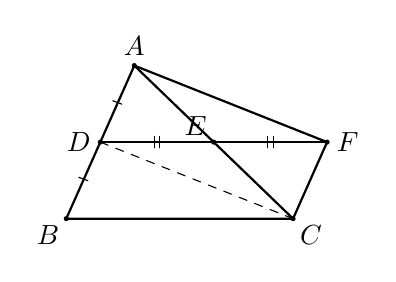
\begin{tikzpicture}[scale=0.72, >=stealth, line join=round, line cap=round]
  \coordinate (B) at (0, 0);
  \coordinate (C) at (4.0, 0);
  \coordinate (A) at (1.2, 2.7);
  \coordinate (D) at (0.6, 1.35);
  \coordinate (E) at (2.6, 1.35);
  \coordinate (F) at (4.6, 1.35);

  \draw[thick] (A) -- (B) -- (C) -- cycle;
  \draw[thick] (D) -- (F);
  \draw[thick] (A) -- (F) -- (C);
  \draw[dashed] (D) -- (C);

  % Vach danh dau trung diem AD = DB
  \draw (0.22, 0.73) -- (0.38, 0.67);
  \draw (0.82, 2.08) -- (0.98, 2.02);

  % Vach danh dau ED = EF
  \draw (1.55, 1.25) -- (1.55, 1.45);
  \draw (1.65, 1.25) -- (1.65, 1.45);
  \draw (3.55, 1.25) -- (3.55, 1.45);
  \draw (3.65, 1.25) -- (3.65, 1.45);

  \fill (A) circle (1.3pt) node[above] {$A$};
  \fill (B) circle (1.3pt) node[below left=-1pt] {$B$};
  \fill (C) circle (1.3pt) node[below right=-1pt] {$C$};
  \fill (D) circle (1.3pt) node[left] {$D$};
  \fill (E) circle (1.3pt) node[above left=-1pt] {$E$};
  \fill (F) circle (1.3pt) node[right] {$F$};
\end{tikzpicture}
\end{minipage}\par
\vspace{0.4mm}
\noindent\textit{Bài giải:}\dongkeHaiCot{11}
\\ \hline
\end{tabularx}

\vspace{1.2mm}

\noindent
\begin{tabularx}{\linewidth}{|X|}
\hline
\vspace{0.5mm}
\textbf{Câu 14 (0,5 điểm).} Tìm giá trị nhỏ nhất của biểu thức: $A = x^2 - 6x + 14$.\par
\vspace{0.4mm}
\noindent\textit{Bài giải:}\dongkeHaiCot{7}
\\ \hline
\end{tabularx}

\newpage
% =============================================================================
% ========================= TOAN 8 TUAN 11 BUOI 01 - MA DE 102 =================
% ========================= TRANG 1/2 ==========================================
% =============================================================================
\noindent
\begin{tabularx}{\linewidth}{|X|c|}
\hline
\textbf{PHIẾU KIỂM TRA ĐỊNH KỲ TOÁN 8 - TUẦN 11 - BUỔI 01} & \textbf{Mã đề: 102 - Trang 1/2} \\
\hline
\end{tabularx}

\vspace{1.0mm}

\noindent
\begin{tabularx}{\linewidth}{|p{3.2cm}|X|}
\hline
\centering\textbf{ĐIỂM SỐ} & \centering\textbf{LỜI NHẬN XÉT CỦA THẦY CÔ} \tabularnewline
\hline
\rule{0pt}{1.8cm} & \tabularnewline
\hline
\end{tabularx}

\vspace{1.2mm}
\noindent\textbf{Câu 1 (0,25 điểm).} Cho $\Delta MNP$ có $E, F$ là trung điểm $MN, MP$. Đoạn thẳng $EF$ là: \shortans{Đường trung bình}\par\vspace{1.8mm}
\noindent\textbf{Câu 2 (0,25 điểm).} Cho $\Delta MNP$ có đường trung bình $EF = 7\text{ cm}$. Độ dài cạnh đáy $NP$ là: \shortans{14\text{ cm}}\par\vspace{1.8mm}
\noindent\textbf{Câu 3 (0,25 điểm).} Cho $\Delta ABC$ có chu vi $30\text{ cm}$. Tam giác nối ba trung điểm có chu vi là: \shortans{15\text{ cm}}\par\vspace{1.8mm}
\noindent\textbf{Câu 4 (0,25 điểm).} Phân tích đa thức $4x^2 - 8x$ thành nhân tử, ta được kết quả là: \shortans{4x(x - 2)}\par\vspace{1.8mm}
\noindent\textbf{Câu 5 (0,25 điểm).} Tính nhanh giá trị của biểu thức $75^2 - 25^2$, ta được kết quả là: \shortans{5\,000}\par\vspace{1.8mm}
\noindent\textbf{Câu 6 (0,25 điểm).} Cho hằng đẳng thức $(x - 4)^2 = x^2 - bx + 16$. Giá trị của hệ số $b$ là: \shortans{8}\par\vspace{1.8mm}
\noindent\textbf{Câu 7 (0,25 điểm).} Bậc của đa thức $Q = 5x^2 y^4 - 3x^3 y^2 + 2$ sau khi thu gọn là: \shortans{6}\par\vspace{1.8mm}
\noindent\textbf{Câu 8 (0,25 điểm).} Cho $x + y = 6$. Giá trị của biểu thức $A = x(x + y) + y(x + y)$ là: \shortans{36}\par\vspace{1.8mm}
\noindent\textbf{Câu 9 (0,25 điểm).} Đo khoảng cách $AB$ qua hồ có ĐTB $MN = 55\text{ m}$. Khi đó $AB$ bằng: \shortans{110\text{ m}}\par\vspace{1.8mm}
\noindent\textbf{Câu 10 (0,25 điểm).} Hình bình hành có một góc vuông là hình gì? \shortans{Hình chữ nhật}\par\vspace{1.8mm}
\vspace{0.2mm}
\noindent\textbf{Câu 11 (3,0 điểm). Phân tích các đa thức sau thành nhân tử:}
\vspace{0.6mm}

\noindent
\begin{tabularx}{\linewidth}{|X|X|}
\hline
\oBaiTap[6]{a) (0,5 điểm)}{$4x^2 - 8x$} & 
\oBaiTap[6]{b) (0,5 điểm)}{$x^2 - 25$} \\
\hline
\oBaiTap[6]{c) (0,5 điểm)}{$x^2 + 8x + 16$} & 
\oBaiTap[6]{d) (0,5 điểm)}{$xy + 3y + 2x + 6$} \\
\hline
\oBaiTap[6]{e) (0,5 điểm)}{$x^2 - 2xy + y^2 - 25$} & 
\oBaiTap[6]{f) (0,5 điểm)}{$x^2 - 7x + 12$} \\
\hline
\end{tabularx}

\newpage
% =============================================================================
% ========================= TOAN 8 TUAN 11 BUOI 01 - MA DE 102 =================
% ========================= TRANG 2/2 ==========================================
% =============================================================================
\noindent
\begin{tabularx}{\linewidth}{|X|c|}
\hline
\textbf{TOÁN 8 - TUẦN 11 - BUỔI 01} & \textbf{Mã đề: 102 - Trang 2/2} \\
\hline
\end{tabularx}

\vspace{1.2mm}

\noindent\textbf{Câu 12 (2,0 điểm). Tìm $x$, biết:}
\vspace{0.6mm}

\noindent
\begin{tabularx}{\linewidth}{|X|X|}
\hline
\oBaiTap[5]{a) (0,5 điểm)}{$x^2 - 5x = 0$} & 
\oBaiTap[5]{b) (0,5 điểm)}{$x^2 - 49 = 0$} \\
\hline
\oBaiTap[5]{c) (0,5 điểm)}{$x^2 - 10x + 25 = 0$} & 
\oBaiTap[5]{d) (0,5 điểm)}{$(x - 1)(x + 4) - 3(x + 4) = 0$} \\
\hline
\end{tabularx}

\vspace{1.2mm}

\noindent
\begin{tabularx}{\linewidth}{|X|}
\hline
\vspace{0.5mm}
\begin{minipage}[t]{0.68\linewidth}
\vspace{0pt}
\textbf{Câu 13 (2,0 điểm).} Cho tam giác $MNP$ nhọn ($MN < MP$). Gọi $D, E$ lần lượt là trung điểm của $MN$ và $MP$.\par\vspace{0.4mm}
\textbf{a)} (1,0 điểm) Chứng minh $DE$ là đường trung bình của tam giác $MNP$. Biết $NP = 14\text{ cm}$, tính độ dài đoạn thẳng $DE$.\par\vspace{0.4mm}
\textbf{b)} (1,0 điểm) Trên tia đối của tia $ED$ lấy điểm $F$ sao cho $EF = ED$. Chứng minh tứ giác $MDFP$ là hình bình hành.
\end{minipage}\hfill
\begin{minipage}[t]{0.30\linewidth}
\vspace{0pt}\centering
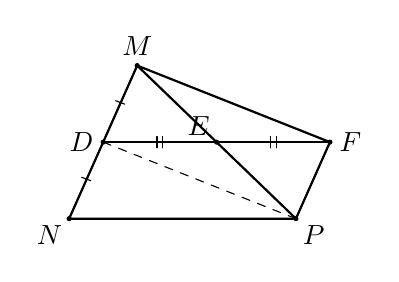
\begin{tikzpicture}[scale=0.72, >=stealth, line join=round, line cap=round]
  \coordinate (N) at (0, 0);
  \coordinate (P) at (4.0, 0);
  \coordinate (M) at (1.2, 2.7);
  \coordinate (D) at (0.6, 1.35);
  \coordinate (E) at (2.6, 1.35);
  \coordinate (F) at (4.6, 1.35);

  \draw[thick] (M) -- (N) -- (P) -- cycle;
  \draw[thick] (D) -- (F);
  \draw[thick] (M) -- (F) -- (P);
  \draw[dashed] (D) -- (P);

  % Vach danh dau trung diem MD = DN
  \draw (0.22, 0.73) -- (0.38, 0.67);
  \draw (0.82, 2.08) -- (0.98, 2.02);

  % Vach danh dau ED = EF
  \draw (1.55, 1.25) -- (1.55, 1.45);
  \draw (1.65, 1.25) -- (1.65, 1.45);
  \draw (3.55, 1.25) -- (3.55, 1.45);
  \draw (3.65, 1.25) -- (3.65, 1.45);

  \fill (M) circle (1.3pt) node[above] {$M$};
  \fill (N) circle (1.3pt) node[below left=-1pt] {$N$};
  \fill (P) circle (1.3pt) node[below right=-1pt] {$P$};
  \fill (D) circle (1.3pt) node[left] {$D$};
  \fill (E) circle (1.3pt) node[above left=-1pt] {$E$};
  \fill (F) circle (1.3pt) node[right] {$F$};
\end{tikzpicture}
\end{minipage}\par
\vspace{0.4mm}
\noindent\textit{Bài giải:}\dongkeHaiCot{11}
\\ \hline
\end{tabularx}

\vspace{1.2mm}

\noindent
\begin{tabularx}{\linewidth}{|X|}
\hline
\vspace{0.5mm}
\textbf{Câu 14 (0,5 điểm).} Tìm giá trị nhỏ nhất của biểu thức: $A = x^2 - 8x + 21$.\par
\vspace{0.4mm}
\noindent\textit{Bài giải:}\dongkeHaiCot{7}
\\ \hline
\end{tabularx}

\newpage
% =============================================================================
% ========================= TOAN 8 TUAN 11 BUOI 01 - MA DE 103 =================
% ========================= TRANG 1/2 ==========================================
% =============================================================================
\noindent
\begin{tabularx}{\linewidth}{|X|c|}
\hline
\textbf{PHIẾU KIỂM TRA ĐỊNH KỲ TOÁN 8 - TUẦN 11 - BUỔI 01} & \textbf{Mã đề: 103 - Trang 1/2} \\
\hline
\end{tabularx}

\vspace{1.0mm}

\noindent
\begin{tabularx}{\linewidth}{|p{3.2cm}|X|}
\hline
\centering\textbf{ĐIỂM SỐ} & \centering\textbf{LỜI NHẬN XÉT CỦA THẦY CÔ} \tabularnewline
\hline
\rule{0pt}{1.8cm} & \tabularnewline
\hline
\end{tabularx}

\vspace{1.2mm}
\noindent\textbf{Câu 1 (0,25 điểm).} Cho $\Delta DEF$ có $I, K$ là trung điểm $DE, DF$. Đoạn thẳng $IK$ là: \shortans{Đường trung bình}\par\vspace{1.8mm}
\noindent\textbf{Câu 2 (0,25 điểm).} Cho $\Delta DEF$ có đường trung bình $IK = 8\text{ cm}$. Độ dài cạnh đáy $EF$ là: \shortans{16\text{ cm}}\par\vspace{1.8mm}
\noindent\textbf{Câu 3 (0,25 điểm).} Cho $\Delta DEF$ có chu vi $28\text{ cm}$. Tam giác nối ba trung điểm có chu vi là: \shortans{14\text{ cm}}\par\vspace{1.8mm}
\noindent\textbf{Câu 4 (0,25 điểm).} Phân tích đa thức $5x^2 - 10x$ thành nhân tử, ta được kết quả là: \shortans{5x(x - 2)}\par\vspace{1.8mm}
\noindent\textbf{Câu 5 (0,25 điểm).} Tính nhanh giá trị của biểu thức $85^2 - 15^2$, ta được kết quả là: \shortans{7\,000}\par\vspace{1.8mm}
\noindent\textbf{Câu 6 (0,25 điểm).} Cho hằng đẳng thức $(2x + 1)^2 = 4x^2 + cx + 1$. Giá trị của hệ số $c$ là: \shortans{4}\par\vspace{1.8mm}
\noindent\textbf{Câu 7 (0,25 điểm).} Bậc của đa thức $R = 2x^5 y - 6x^2 y^3 + 9$ sau khi thu gọn là: \shortans{6}\par\vspace{1.8mm}
\noindent\textbf{Câu 8 (0,25 điểm).} Cho $x + y = 7$. Giá trị của biểu thức $A = x(x + y) + y(x + y)$ là: \shortans{49}\par\vspace{1.8mm}
\noindent\textbf{Câu 9 (0,25 điểm).} Đo khoảng cách $AB$ qua hồ có ĐTB $MN = 38\text{ m}$. Khi đó $AB$ bằng: \shortans{76\text{ m}}\par\vspace{1.8mm}
\noindent\textbf{Câu 10 (0,25 điểm).} Hình bình hành có hai cạnh kề bằng nhau là hình gì? \shortans{Hình thoi}\par\vspace{1.8mm}
\vspace{0.2mm}
\noindent\textbf{Câu 11 (3,0 điểm). Phân tích các đa thức sau thành nhân tử:}
\vspace{0.6mm}

\noindent
\begin{tabularx}{\linewidth}{|X|X|}
\hline
\oBaiTap[6]{a) (0,5 điểm)}{$5x^2 - 15x$} & 
\oBaiTap[6]{b) (0,5 điểm)}{$4x^2 - 9$} \\
\hline
\oBaiTap[6]{c) (0,5 điểm)}{$x^2 - 10x + 25$} & 
\oBaiTap[6]{d) (0,5 điểm)}{$xy + 4y + 2x + 8$} \\
\hline
\oBaiTap[6]{e) (0,5 điểm)}{$x^2 + 2xy + y^2 - 9$} & 
\oBaiTap[6]{f) (0,5 điểm)}{$x^2 + 5x + 6$} \\
\hline
\end{tabularx}

\newpage
% =============================================================================
% ========================= TOAN 8 TUAN 11 BUOI 01 - MA DE 103 =================
% ========================= TRANG 2/2 ==========================================
% =============================================================================
\noindent
\begin{tabularx}{\linewidth}{|X|c|}
\hline
\textbf{TOÁN 8 - TUẦN 11 - BUỔI 01} & \textbf{Mã đề: 103 - Trang 2/2} \\
\hline
\end{tabularx}

\vspace{1.2mm}

\noindent\textbf{Câu 12 (2,0 điểm). Tìm $x$, biết:}
\vspace{0.6mm}

\noindent
\begin{tabularx}{\linewidth}{|X|X|}
\hline
\oBaiTap[5]{a) (0,5 điểm)}{$x^2 + 3x = 0$} & 
\oBaiTap[5]{b) (0,5 điểm)}{$x^2 - 81 = 0$} \\
\hline
\oBaiTap[5]{c) (0,5 điểm)}{$x^2 + 6x + 9 = 0$} & 
\oBaiTap[5]{d) (0,5 điểm)}{$(x - 3)(x + 2) - 2(x + 2) = 0$} \\
\hline
\end{tabularx}

\vspace{1.2mm}

\noindent
\begin{tabularx}{\linewidth}{|X|}
\hline
\vspace{0.5mm}
\begin{minipage}[t]{0.68\linewidth}
\vspace{0pt}
\textbf{Câu 13 (2,0 điểm).} Cho tam giác $ABC$ nhọn ($AB < AC$). Gọi $M, N$ lần lượt là trung điểm của $AB$ và $AC$.\par\vspace{0.4mm}
\textbf{a)} (1,0 điểm) Chứng minh $MN$ là đường trung bình của tam giác $ABC$. Biết $BC = 16\text{ cm}$, tính độ dài đoạn thẳng $MN$.\par\vspace{0.4mm}
\textbf{b)} (1,0 điểm) Trên tia đối của tia $NM$ lấy điểm $P$ sao cho $NP = NM$. Chứng minh tứ giác $AMCP$ là hình bình hành.
\end{minipage}\hfill
\begin{minipage}[t]{0.30\linewidth}
\vspace{0pt}\centering
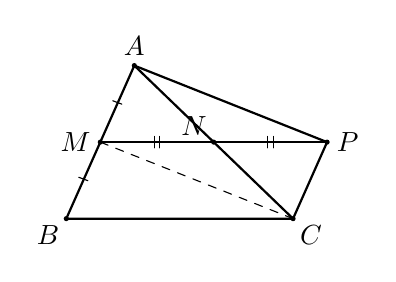
\begin{tikzpicture}[scale=0.72, >=stealth, line join=round, line cap=round]
  \coordinate (B) at (0, 0);
  \coordinate (C) at (4.0, 0);
  \coordinate (A) at (1.2, 2.7);
  \coordinate (M) at (0.6, 1.35);
  \coordinate (N) at (2.6, 1.35);
  \coordinate (P) at (4.6, 1.35);

  \draw[thick] (A) -- (B) -- (C) -- cycle;
  \draw[thick] (M) -- (P);
  \draw[thick] (A) -- (P) -- (C);
  \draw[dashed] (M) -- (C);

  % Vach danh dau trung diem AM = MB
  \draw (0.22, 0.73) -- (0.38, 0.67);
  \draw (0.82, 2.08) -- (0.98, 2.02);

  % Vach danh dau NM = NP
  \draw (1.55, 1.25) -- (1.55, 1.45);
  \draw (1.65, 1.25) -- (1.65, 1.45);
  \draw (3.55, 1.25) -- (3.55, 1.45);
  \draw (3.65, 1.25) -- (3.65, 1.45);

  \fill (A) circle (1.3pt) node[above] {$A$};
  \fill (B) circle (1.3pt) node[below left=-1pt] {$B$};
  \fill (C) circle (1.3pt) node[below right=-1pt] {$C$};
  \fill (M) circle (1.3pt) node[left] {$M$};
  \fill (N) circle (1.3pt) node[above left=-1pt] {$N$};
  \fill (P) circle (1.3pt) node[right] {$P$};
\end{tikzpicture}
\end{minipage}\par
\vspace{0.4mm}
\noindent\textit{Bài giải:}\dongkeHaiCot{11}
\\ \hline
\end{tabularx}

\vspace{1.2mm}

\noindent
\begin{tabularx}{\linewidth}{|X|}
\hline
\vspace{0.5mm}
\textbf{Câu 14 (0,5 điểm).} Tìm giá trị nhỏ nhất của biểu thức: $A = x^2 - 4x + 11$.\par
\vspace{0.4mm}
\noindent\textit{Bài giải:}\dongkeHaiCot{7}
\\ \hline
\end{tabularx}

\newpage
% =============================================================================
% ========================= TOAN 8 TUAN 11 BUOI 01 - MA DE 104 =================
% ========================= TRANG 1/2 ==========================================
% =============================================================================
\noindent
\begin{tabularx}{\linewidth}{|X|c|}
\hline
\textbf{PHIẾU KIỂM TRA ĐỊNH KỲ TOÁN 8 - TUẦN 11 - BUỔI 01} & \textbf{Mã đề: 104 - Trang 1/2} \\
\hline
\end{tabularx}

\vspace{1.0mm}

\noindent
\begin{tabularx}{\linewidth}{|p{3.2cm}|X|}
\hline
\centering\textbf{ĐIỂM SỐ} & \centering\textbf{LỜI NHẬN XÉT CỦA THẦY CÔ} \tabularnewline
\hline
\rule{0pt}{1.8cm} & \tabularnewline
\hline
\end{tabularx}

\vspace{1.2mm}
\noindent\textbf{Câu 1 (0,25 điểm).} Cho $\Delta ABC$ có $D, E$ là trung điểm $AB, BC$. Đoạn thẳng $DE$ là: \shortans{Đường trung bình}\par\vspace{1.8mm}
\noindent\textbf{Câu 2 (0,25 điểm).} Cho $\Delta MNP$ có đường trung bình $EF = 9\text{ cm}$. Độ dài cạnh đáy $NP$ là: \shortans{18\text{ cm}}\par\vspace{1.8mm}
\noindent\textbf{Câu 3 (0,25 điểm).} Cho $\Delta MNP$ có chu vi $36\text{ cm}$. Tam giác nối ba trung điểm có chu vi là: \shortans{18\text{ cm}}\par\vspace{1.8mm}
\noindent\textbf{Câu 4 (0,25 điểm).} Phân tích đa thức $2x^2 - 6x$ thành nhân tử, ta được kết quả là: \shortans{2x(x - 3)}\par\vspace{1.8mm}
\noindent\textbf{Câu 5 (0,25 điểm).} Tính nhanh giá trị của biểu thức $95^2 - 5^2$, ta được kết quả là: \shortans{9\,000}\par\vspace{1.8mm}
\noindent\textbf{Câu 6 (0,25 điểm).} Cho hằng đẳng thức $(x + 5)^2 = x^2 + dx + 25$. Giá trị của hệ số $d$ là: \shortans{10}\par\vspace{1.8mm}
\noindent\textbf{Câu 7 (0,25 điểm).} Bậc của đa thức $T = 7xy^5 - 4x^3 y^2 + 5$ sau khi thu gọn là: \shortans{6}\par\vspace{1.8mm}
\noindent\textbf{Câu 8 (0,25 điểm).} Cho $x + y = 8$. Giá trị của biểu thức $A = x(x + y) + y(x + y)$ là: \shortans{64}\par\vspace{1.8mm}
\noindent\textbf{Câu 9 (0,25 điểm).} Đo khoảng cách $AB$ qua hồ có ĐTB $MN = 62\text{ m}$. Khi đó $AB$ bằng: \shortans{124\text{ m}}\par\vspace{1.8mm}
\noindent\textbf{Câu 10 (0,25 điểm).} Hình chữ nhật có hai cạnh kề bằng nhau là hình gì? \shortans{Hình vuông}\par\vspace{1.8mm}
\vspace{0.2mm}
\noindent\textbf{Câu 11 (3,0 điểm). Phân tích các đa thức sau thành nhân tử:}
\vspace{0.6mm}

\noindent
\begin{tabularx}{\linewidth}{|X|X|}
\hline
\oBaiTap[6]{a) (0,5 điểm)}{$2x^2 - 8x$} & 
\oBaiTap[6]{b) (0,5 điểm)}{$9x^2 - 16$} \\
\hline
\oBaiTap[6]{c) (0,5 điểm)}{$x^2 + 12x + 36$} & 
\oBaiTap[6]{d) (0,5 điểm)}{$xy + 5y + 3x + 15$} \\
\hline
\oBaiTap[6]{e) (0,5 điểm)}{$x^2 + 2xy + y^2 - 49$} & 
\oBaiTap[6]{f) (0,5 điểm)}{$x^2 - 8x + 15$} \\
\hline
\end{tabularx}

\newpage
% =============================================================================
% ========================= TOAN 8 TUAN 11 BUOI 01 - MA DE 104 =================
% ========================= TRANG 2/2 ==========================================
% =============================================================================
\noindent
\begin{tabularx}{\linewidth}{|X|c|}
\hline
\textbf{TOÁN 8 - TUẦN 11 - BUỔI 01} & \textbf{Mã đề: 104 - Trang 2/2} \\
\hline
\end{tabularx}

\vspace{1.2mm}

\noindent\textbf{Câu 12 (2,0 điểm). Tìm $x$, biết:}
\vspace{0.6mm}

\noindent
\begin{tabularx}{\linewidth}{|X|X|}
\hline
\oBaiTap[5]{a) (0,5 điểm)}{$x^2 + 6x = 0$} & 
\oBaiTap[5]{b) (0,5 điểm)}{$x^2 - 64 = 0$} \\
\hline
\oBaiTap[5]{c) (0,5 điểm)}{$x^2 + 10x + 25 = 0$} & 
\oBaiTap[5]{d) (0,5 điểm)}{$(x - 2)(x + 5) - 3(x + 5) = 0$} \\
\hline
\end{tabularx}

\vspace{1.2mm}

\noindent
\begin{tabularx}{\linewidth}{|X|}
\hline
\vspace{0.5mm}
\begin{minipage}[t]{0.68\linewidth}
\vspace{0pt}
\textbf{Câu 13 (2,0 điểm).} Cho tam giác $DEF$ nhọn ($DE < DF$). Gọi $M, N$ lần lượt là trung điểm của $DE$ và $DF$.\par\vspace{0.4mm}
\textbf{a)} (1,0 điểm) Chứng minh $MN$ là đường trung bình của tam giác $DEF$. Biết $EF = 18\text{ cm}$, tính độ dài đoạn thẳng $MN$.\par\vspace{0.4mm}
\textbf{b)} (1,0 điểm) Trên tia đối của tia $NM$ lấy điểm $P$ sao cho $NP = NM$. Chứng minh tứ giác $DMFP$ là hình bình hành.
\end{minipage}\hfill
\begin{minipage}[t]{0.30\linewidth}
\vspace{0pt}\centering
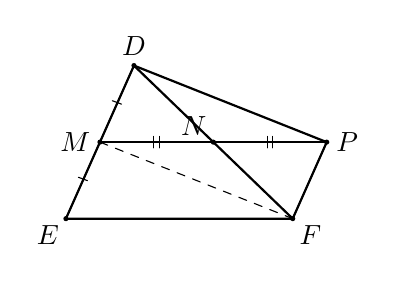
\begin{tikzpicture}[scale=0.72, >=stealth, line join=round, line cap=round]
  \coordinate (E) at (0, 0);
  \coordinate (F) at (4.0, 0);
  \coordinate (D) at (1.2, 2.7);
  \coordinate (M) at (0.6, 1.35);
  \coordinate (N) at (2.6, 1.35);
  \coordinate (P) at (4.6, 1.35);

  \draw[thick] (D) -- (E) -- (F) -- cycle;
  \draw[thick] (M) -- (P);
  \draw[thick] (D) -- (P) -- (F);
  \draw[dashed] (M) -- (F);

  % Vach danh dau trung diem DM = ME
  \draw (0.22, 0.73) -- (0.38, 0.67);
  \draw (0.82, 2.08) -- (0.98, 2.02);

  % Vach danh dau NM = NP
  \draw (1.55, 1.25) -- (1.55, 1.45);
  \draw (1.65, 1.25) -- (1.65, 1.45);
  \draw (3.55, 1.25) -- (3.55, 1.45);
  \draw (3.65, 1.25) -- (3.65, 1.45);

  \fill (D) circle (1.3pt) node[above] {$D$};
  \fill (E) circle (1.3pt) node[below left=-1pt] {$E$};
  \fill (F) circle (1.3pt) node[below right=-1pt] {$F$};
  \fill (M) circle (1.3pt) node[left] {$M$};
  \fill (N) circle (1.3pt) node[above left=-1pt] {$N$};
  \fill (P) circle (1.3pt) node[right] {$P$};
\end{tikzpicture}
\end{minipage}\par
\vspace{0.4mm}
\noindent\textit{Bài giải:}\dongkeHaiCot{11}
\\ \hline
\end{tabularx}

\vspace{1.2mm}

\noindent
\begin{tabularx}{\linewidth}{|X|}
\hline
\vspace{0.5mm}
\textbf{Câu 14 (0,5 điểm).} Tìm giá trị nhỏ nhất của biểu thức: $A = x^2 - 10x + 31$.\par
\vspace{0.4mm}
\noindent\textit{Bài giải:}\dongkeHaiCot{7}
\\ \hline
\end{tabularx}
\end{document}
